\subsection{System Context}
\label{subsec:requirements}
\begin{figure}[ht]
    \centering
    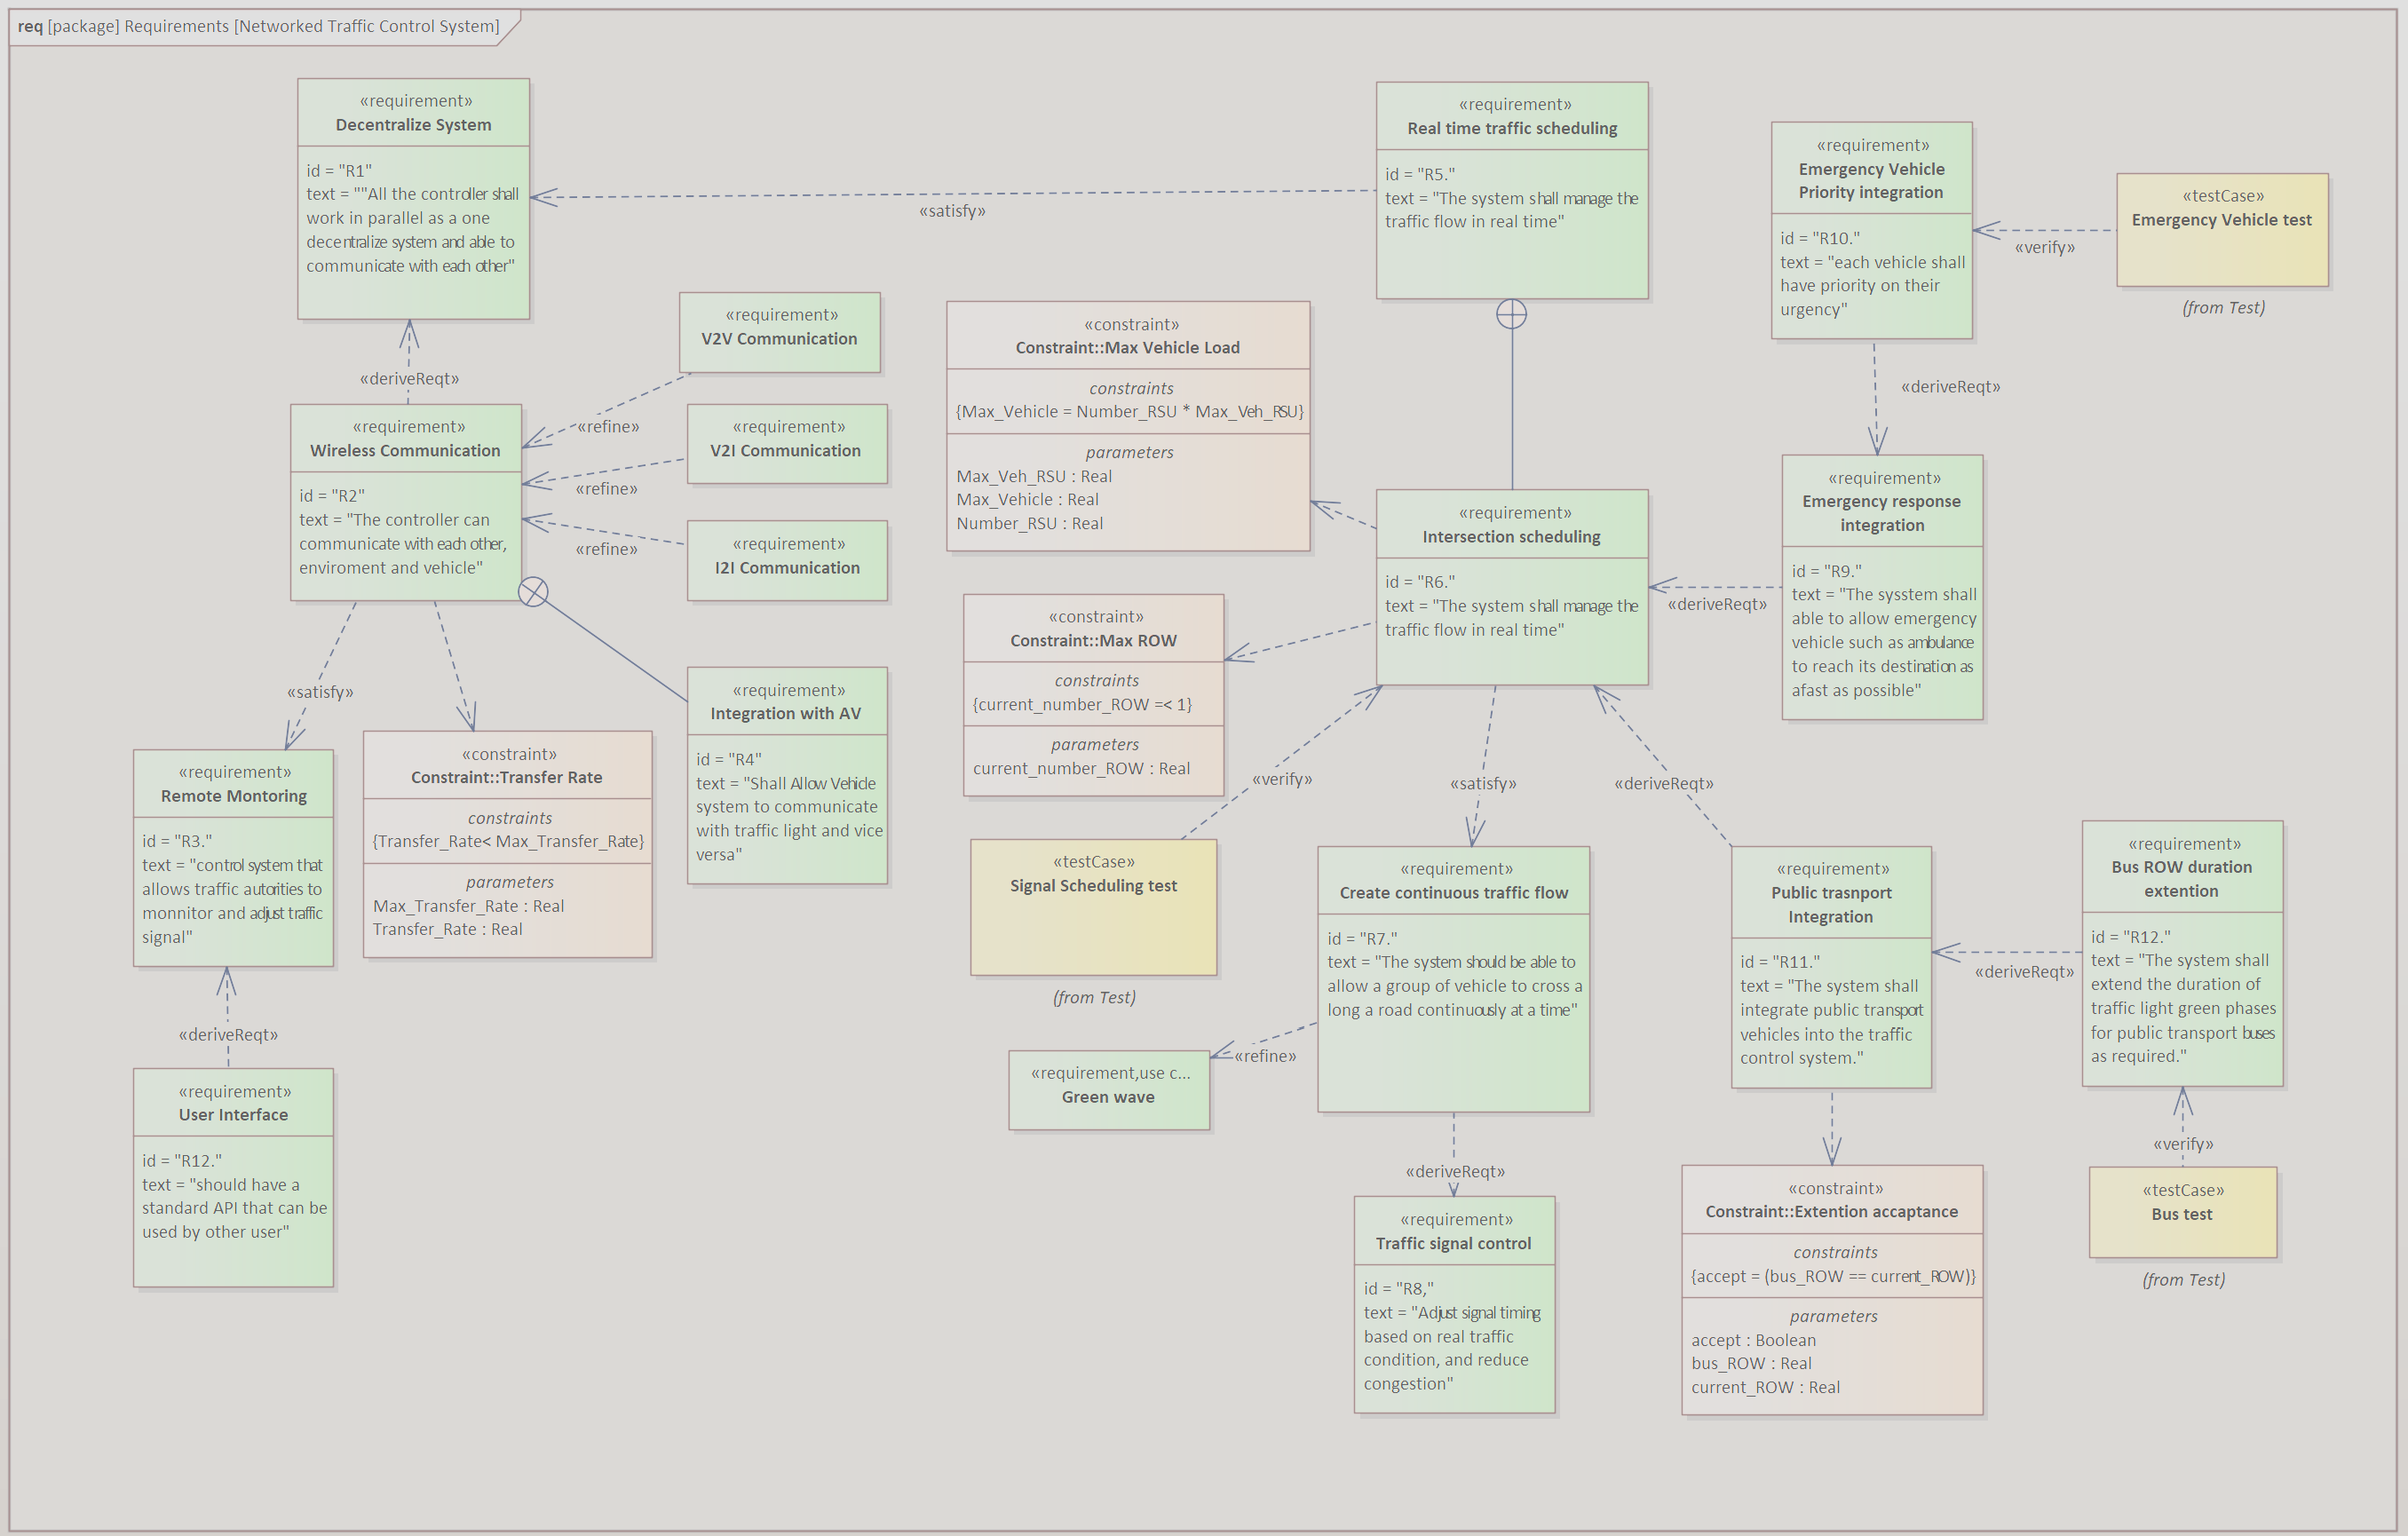
\includegraphics[width=0.5\textwidth]{images/requirements.png}
    \caption{Requirements Diagram}
    \label{img:system_bdd}
\end{figure}
The system requirements diagram in Figure \ref{img:system_bdd} describes the relationship between different requirements blocks and system constraints. The system requires all controllers to communicate and work together as a decentralized system; therefore, the system should have wireless communication capabilities and should support vehicle-to-vehicle, vehicle-to-infrastructure, and infrastructure-to-infrastructure communication. It should satisfy remote traffic monitoring. It must schedule traffic at intersections, prioritize public transportation, communicate with emergency vehicles, and schedule pedestrian crossings in real-time. It should also prioritize emergency vehicle access to the intersection.